\documentclass{llncs}
\usepackage{url}
\usepackage{proof}
\usepackage{amssymb}
\usepackage{stmaryrd}
\usepackage{listings}
\usepackage{graphicx}

\newcommand{\todo}[1]{\textbf{TODO: #1}}

%subcode-inline{bnf-inline} name langRev
%! swap+ = \mathit{swap}^+
%! swap* = \mathit{swap}^*
%! dagger =  ^{\dagger}
%! assocl+ = \mathit{assocl}^+
%! assocr+ = \mathit{assocr}^+
%! assocl* = \mathit{assocl}^*
%! assocr* = \mathit{assocr}^*
%! identr* = \mathit{uniti}
%! identl* = \mathit{unite}
%! dist = \mathit{distrib}
%! factor = \mathit{factor}
%! (o) = \fatsemi
%! (;) = \fatsemi
%! (*) = \times
%! (+) = +


%subcode-inline{bnf-inline} regex \{\{(((\}[^\}])|[^\}])*)\}\} name main include langRev
%! |-->* = \mapsto^{*}
%! |-->> = \mapsto_{\ggg}
%! |-->let = \mapsto_{let}
%! |--> = \mapsto
%! |- = \vdash
%! in = \!\!\in\!\!
%! <=> = \Longleftrightarrow
%! <-> = \leftrightarrow
%! ~> = \leadsto
%! ::= = ::=
%! /= = \neq
%! vi = v_i
%! di = d_i
%! si = s_i
%! sj = s_j
%! F = \texttt{F}
%! T = \texttt{T}
%! forall = \forall
%! exists = \exists
%! empty = \emptyset
%! eta = \eta
%! where = \textbf{where}
%! epsilon = \varepsilon
%! least = \phi
%! trace+ = trace
%! trace* = trace_{\times}
%! loop+ = loop_{+}
%! loop* = loop_{\times}
%! CatC = {\mathcal C}
%! CatA = {\mathcal A}
%! gamma = \gamma
%! {[ = \{
%! ]} = \}
%! elem = \in
%! dagger = ^\dagger
%! alpha = \alpha
%! beta = \beta
%! rho = \rho
%! @@ = \mu
%! @ = \,@\,
%! langRev = \Pi
%! langRevT = \Pi^{o}
%! bullet = \bullet
%! * = \times

\urldef{\mails}\path|{rpjames, sabry}@indiana.edu|

%%%%%%%%%%%%%%%%%%%%%%%%%%%%%%%%%%%%%%%%%%%%%%%%%%%%%%%%%%%%%%%%%%%%%%%%%%%%%

\begin{document}
\title{On the Construction of Isomorphic Interpreters} 
\titlerunning{On the construction of Isomorphic Interpreters} 
\author{Roshan P. James \and Amr Sabry}
\institute{School of Informatics and Computing, Indiana University\\
\mails}
\maketitle

%%%%%%%%%%%%%%%%%%%%%%%%%%%%%%%%%%%%%%%%%%%%%%%%%%%%%%%%%%%%%%%%%%%%%%%%%%%%%
\begin{abstract}
\end{abstract}

%%%%%%%%%%%%%%%%%%%%%%%%%%%%%%%%%%%%%%%%%%%%%%%%%%%%%%%%%%%%%%%%%%%%%%%%%%%%%
\section{Introduction} 

The constructions in this paper apply only to a class of interpreters
that can be represented by logically reversible small-step operational
semantics. While, in a formal sense, they are related to Abramsky's
``bi-orthogonal automata'' , we will try to give them a more direct
characterization purely in terms of logical reversibility of the
small-step semantics.


\section{Simple Bounded Iterator}
Consider definition for the following small-step abstract machine:

%subcode{bnf} include main
% Expressions, e = n
% Numbers, n, m = 0 | n + 1
%
% Machine states = <e, e>
% Start state = <n, 0>
% Stop State = <0, n>

Small-step Operational semantics:

%subcode{opsem} include main
% <n+1, m> |--> <n, m+1>

This machine start with a number {{n}} in the first position and at
each reduction step decrements the first number and increments the
second. It stops when the first number reaches 0, thereby taking
exactly {{n}} steps. While the machine does nothing interesting,
it useful to illustrate the general idea.

We can turn this abstract machine into a an isomorphic interpreter
implemented in {{langRevT}}, in a systematic way. To start with we
realize that the interpreter should implement the following map.

\begin{center}
  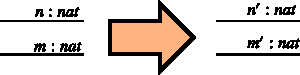
\includegraphics{diagrams/nat-nat1.pdf}
\end{center}

Now numbers can be implemented by the recursive type {{nat = @@x.1+x}}
in {{langRevT}}. This gives us the isomorphisms 

\begin{center}
  {{unfold : nat <-> 1 + nat : fold}}
\end{center}

We start by examining the first value. 

\begin{center}
  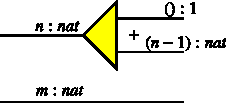
\includegraphics{diagrams/nat-nat2.pdf}
\end{center}

The triangle denotes the {{unfold}} isomorphism, which works as
follows: If the number {{n}} is zero, the output is the top branch
which has type {{1}}. If the number was non-zero, the output is on the
bottom branch and has value {{n-1}}. 

Since the abstract machine increments second component, we know that
we need a {{fold}} on the second component to accomplish this. So we
can fill in the output part of the interpreter dually. 

\begin{center}
  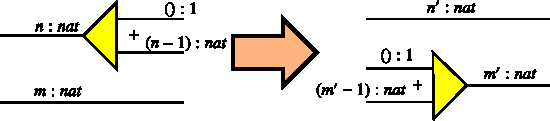
\includegraphics{diagrams/nat-nat3.pdf}
\end{center}

Let us examine all the possible input states, by distributing on the
input. Dually let us do the same with the output, but this time also
be a little bit explicit about the swap operations required so the
right types are in place.

\begin{center}
  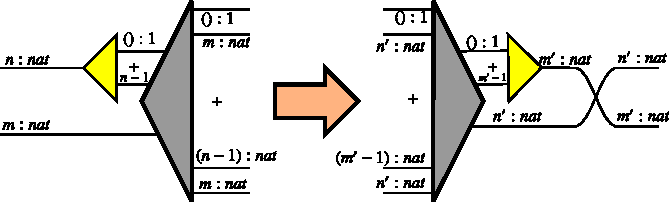
\includegraphics{diagrams/nat-nat4.pdf}
\end{center}

The construction above already gives us some insight into how we can
implement our one reduction step. If we chose {{m = m'-1}} and we
chose {{n-1 =n'}} then we have essentially encoded the required
rewrite. Lets state this in words - the new value of {{n}}, namely
{{n'}}, is equal to {{n-1}}. And further - the new value of {{m}},
namely {{m'}}, is {{m+1}} (because {{m'-1=m}}). 

We can thus connect the lower branches with the appropriate
isomorphism to reflect this relationship. In this case the isomorphism
is just a swap of the two wires involved.

\begin{center}
  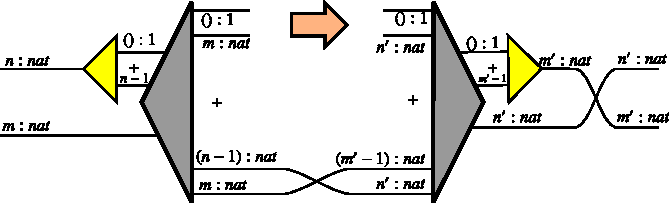
\includegraphics{diagrams/nat-nat5.pdf}
\end{center}

We are a few steps away from an interpreter at this point and the
final steps rely on the answers to a few questions.

\begin{enumerate}
\item How do relate the outputs of the combinator to the inputs, such
  that the machine correctly takes multiple steps?

\item What do we do about the two inner branches? 

\end{enumerate}

The branch labelled {{((), m)}} looks like the stop state of the
machine. The branch labelled {{((), n')}} looks like the start state
of the program. To complete the interpreter, we flip our current
construction inside out.

\begin{center}
  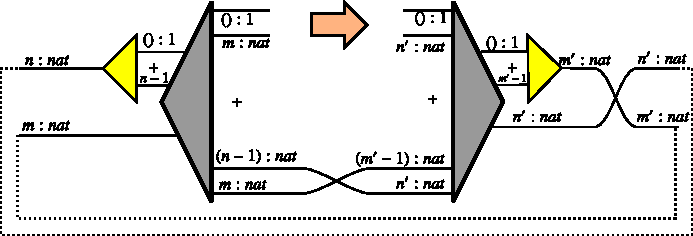
\includegraphics{diagrams/nat-nat6.pdf}
\end{center}

Which gives us

\begin{center}
  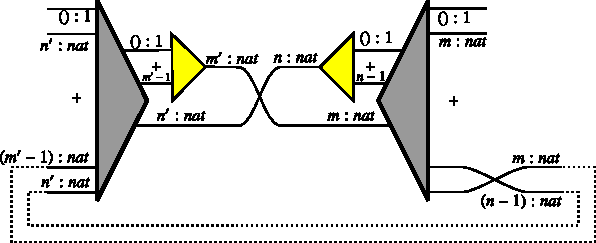
\includegraphics{diagrams/nat-nat7.pdf}
\end{center}

This basically completely our construction of the interpreter. We
basically need to use a {{trace}} to feedback related machine states
to related machine states.

\begin{center}
  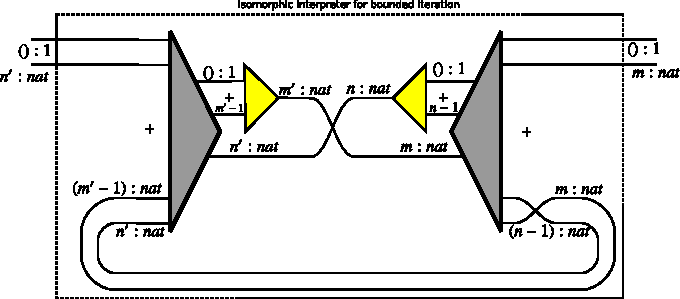
\includegraphics{diagrams/nat-nat8.pdf}
\end{center}

%%%%%%%%%%%%%%%%%%%%%%%%%%%%%%%%%%%%%%%%%%%%%%%%%%%%%%%%%%%%%%%%%%%%%%%%%%%%%%%%%%%%%
\section{Abstracting out the Construction}



%%%%%%%%%%%%%%%%%%%%%%%%%%%%%%%%%%%%%%%%%%%%%%%%%%%%%%%%%%%%%%%%%%%%%%%%%%%%%%%%%%%%%
\section{Adder and Multiplier}

%%%%%%%%%%%%%%%%%%%%%%%%%%%%%%%%%%%%%%%%%%%%%%%%%%%%%%%%%%%%%%%%%%%%%%%%%%%%%%%%%%%%%
\section{Tree Traversal}





\bibliographystyle{splncs03} 
\bibliography{cites}
\end{document}

